\documentclass[runningheads]{llncs}
%
\usepackage{graphicx}
\usepackage{amsmath}
\usepackage{amssymb}
\usepackage{stmaryrd}
\usepackage{listings}
\usepackage{bussproofs}
\usepackage{graphicx}
\usepackage{minted}
\usepackage{tikz}
\usepackage[title]{appendix}

\makeatletter
\newcommand{\@chapapp}{\relax}%
\makeatother

\begin{document}
%
\title{Project Report on DeepSpecDB}

\author{Yixuan Chen\inst{1}}
\institute{University of Michigan}
\maketitle

\begin{abstract}
  Recent years have witnessed a rapid development of main-memory database
  systems thanks to the growingly affordable memory. DeepSpecDB is another
  main-memory database management system implemented in C with deep
  specification and end-to-end verification guaranteeing the correctness of the
  system.
\end{abstract}

\section{Introduction}

As the unit price of memory decreases over time, efforts have been put into
migrating the traditional disk-based applications into main memory. A classical
category of such applications are databases. For example, H-store~\cite{hstore},
MongoDB, Redis and Memcached are well-known database systems featuring
main-memory index and storage.

Meanwhile, database systems are usually barely specified and vulnerable to
subtle bugs. We believe that verified programs against deep specification is the
remedy for the database. Deep specification will ensure that the behavior will
be captured by the specification and proven correctly by machine-checked proof.
With the help of the Verified Software Toolchain~\cite{VST}, we are now able to
verify C programs against the C11 operational semantics. The DeepSpecDB project
aims to develop a main-memory database system with deep specification
guaranteeing the correctness of the system. 

One of the previous development of main-memory database is
MassTree~\cite{masstree}. MassTree implements the \textit{trie over B+ tree} 
style key-value store for keys of variable length strings. The data-structure is
specially tailored for the cache of modern day processors. The original MassTree
is designed for single-key transactions, but later development of
Silo~\cite{Silo} and SiloR~\cite{SiloR} suggest its capability of indexing for
relational databases.

The index engine for databases is basically a mapping from index to rows.
Additionally, to support iterations and optimize bulk operations we need a way
to traverse through the index. For this purpose, a data structure called
\textit{Cursor} is introduced. A cursor is a thread-local object that points to
position inside some indexing data structure and supports local movements and
operations. MassTree supports cursors with minor modification to the data
structure, and is chosen to be the indexing data structure of variable length
strings in DeepSpecDB project.

Before my work, Aur\`ele Barri\`ere~\cite{aurele} has already verified the
correspondence between functional and C implementation of B+ tree with cursors.
Brian McSwiggen~\cite{brian} has developed a specification of B+ tree with
cursors. Oluwatosin Victor Adewale~\cite{oluwatosin} has developed the C
implementation for MassTree, however, the cursor for trie is not implemented.

In this report, I present my work on verification of trie with cursors. In
Section~\ref{modver}, I will present the methods I use in verification and the
reason behind them. In Section~\ref{spec}, I will discuss about the
specification we derived so far for any data structures with cursors. In
Section~\ref{trie}, I will introduce the instantiation of the specification with
trie as internal data structures. In Section~\ref{walkthrough}, I will walk
through a client routine for the indexing data structure, and present what the
end-to-end verification guarantee. 

\section{Terminology}

In this report, I will use the term \emph{kv-map} (stands for key-value map) for
data structures that supports \texttt{put} and \texttt{get} operations similar
to a finite map. 

% In this report, I will use the term \emph{table} for data structures that
% supports \texttt{put} and \texttt{get} operations the same way as a finite map
% (this is not a proper term in larger context of the database, and it's a
% historical issue should be resolved soon).

\section{Modular Verification}\label{modver}

Modularity is the way to achieve scalability. In this section, I will discuss
about the efforts in modularizing the verification, and present an overview
of the verification structure of the project.

\begin{figure}[htbp]
  \centering
  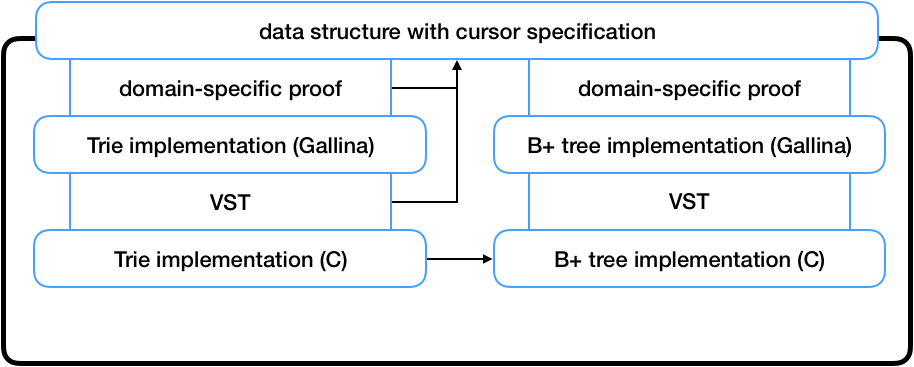
\includegraphics[width=\textwidth]{diagram.png}
  \caption{Verification Structure}\label{fig:struct}
\end{figure}

\subsection{Functional Specification of C Programs}

When verifying a C program against specification, there are generally two
approaches. One is to prove the specification directly within separation
logic. The other is to prove that the C program refines a functional program,
and the functional program is proved later to satisfy the specification. We
favor the latter method.

The functional specification modularizes the verification, and therefore
is beneficial in several aspects. When verifying the C program, we would never
want to deal with application-domain theories accompanied with low level
details in separation logic. By elevating the C program into functional
programs, we are decoupling the refinement proof from the property proofs, and
both proofs are easier and more maintainable. Meanwhile, it turns out that
deriving the perfect specification the first time is almost impossible: The
specification evolves as we are verifying the program. Without a functional
program in between, we will have to rewrite the entire proof. However, the
functional program usually captures all observable behaviors, and therefore the
refinement proof usually remains unchanged. Similarly, while the C program might
be modified for bug fixes, only the lower part of proof needs review, while the
application domain reasoning stays valid.

Concretely in this project, both the B+ trees and tries are implemented in C as
well as in Gallina, where the refinement relation between the two programs is
established using Verified Software Toolchain. After establishing the refinement
relation, we focus mainly on the functional programs for later verification.

\subsection{Modularizing the Components}

Using the functional programs is an effort to modularize the verification
vertically, we would also like to modularize horizontally. In this project,
indexing of database systems are separated from the other parts. Therefore it
naturally forms a verification boundary: Any indexing data structure will
implement a uniform specification, the only part exposed to the rest of the
project. As shown in figure~\ref{fig:struct}, everything surrounded in the bold
square is opaque to the rest of project, while the only interface is the
specification.

Within the index engine, MassTree is naturally divided into two modules: A
module that implements B+ tree with cursors and a module that relies on previous
module to implement trie with cursors. In the verification of trie, we went a
further step where we parameterized over the dependency: for any module that
implements the specification of kv-map of integer-typed key with
cursors, we can derive a module that implements the same specification of
string-typed key with cursors using the trie data structure. Such
parameterization modularized the verification in the way that verification of
trie is now independent from any detail in implementation or verification of B+
trees. Also as a side effect, this approach \textbf{tested} the
\textit{two-sidedness} of the specification: As a consumer of the specification,
a successful verification implied that the specification was sufficient in
capturing the behaviors. Meanwhile as a provider, it made sure that only
reasonable properties was specified.

In Coq, this modularization is achieved through \texttt{Module} and
\texttt{Module Type}. The specification is expressed as a \texttt{Module Type}
where interface functions are expressed as parameters and properties are
expressed as axioms. A \texttt{Module} can implement a \texttt{Module Type} by
providing all the parameters and justifying all the axioms. The dependency of
modules are expressed as functors.

\section{Specification for KV-Map with Cursors}\label{spec}

In this section I will introduce the specification for indexing data
structures. The specification can be generally divided into two parts: the part
where it guaranteed the correctness of the kv-map itself and the part where it
provided essential utilities for clients' reasoning.

\subsection{Interface}

Spiritually, a kv-map maintains the mapping from keys to values and a cursor
points into the kv-map at a specific position and supports movement operations.
Concretely, such a data structure should provide the operations in
figure~\ref{fig:interface}.

\begin{figure}[htbp]
  \centering
  \begin{minted}{coq}
Module Type KV_MAP (KeyType: UsualOrderedType).
  Definition key := KeyType.t.
  Parameter map: Type -> Type.
  Parameter cursor: Type -> Type.

  Section Types.
    Context {value: Type}.
    Parameter empty: map value -> Prop.

    Parameter make_cursor: key -> map value -> cursor value.
    Parameter first_cursor: map value -> cursor value.
    Parameter last_cursor: map value -> cursor value.
    Parameter next_cursor: cursor value -> map value -> cursor value.
    Parameter prev_cursor: cursor value -> map value -> cursor value.
    
    Parameter get: cursor value -> map value -> option (key * value).

    Parameter put: key -> value -> cursor value -> map value -> (* input *)
                   cursor value -> map value -> (* output *)
                   Prop.
    [...]
  End Types.
End KV_MAP.
\end{minted}
  \caption{Interface for KV-Map with Cursors}\label{fig:interface}
\end{figure}

This is a typical interface of kv-map which supports operations for creation of
map (\texttt{empty}), creation of cursor (\texttt{make\_cursor},
\texttt{first\_cursor}, \texttt{last\_cursor}), movement of cursor
(\texttt{next\_cursor}, \texttt{prev\_cursor}), fetching data at
cursor (\texttt{get}) and updating the map (\texttt{put}). The types of
functions indicates clearly that all other functions except for \texttt{empty}
and \texttt{put} are immutable with respect to the map. The two map mutating
functions are defined as relations rather than functions, this is a compromise
to support cursors. I will discuss the reason and consequence of relational
specification in detail later in this section.

Apart from these functions, we also need some auxiliary predicates, as shown in
figure~\ref{fig:aux}. \texttt{abs\_rel} asserts that a cursor and a kv-map are
correctly associated with each other (the abbreviation \texttt{abs} should
stands for \emph{abstraction}, but it's not a right word here, rather a
historical issue). \texttt{key\_rel} asserts that a cursor is associated with
a key in a kv-map. One can imagine this predicate as \textit{the cursor is placed
at the position such that all the existing keys to the decreasing side are less
than this key, and all the existing keys to the opposite are no less than this
key}. This makes sense when one visualizes a kv-map as a list of pairs of key and
value. This definition is closely related to the semantics of \texttt{get}, We
will see later how this is used in generalized kv-map. \texttt{eq\_cursor}
asserts that two cursors are equivalent. Coq equality (\texttt{eq}) does not
work well here, because of \texttt{eq} implies structural equality, and
structurally different cursors can be equivalent (especially for those kv-map
with complex structures, such as B+ trees or tries). The final two predicates
\texttt{cursor\_correct} and \texttt{map\_correct} are the normal invariants.

\begin{figure}[htbp]
  \centering
  \begin{minted}{coq}
Module Type KV_MAP (KeyType: UsualOrderedType).
  [...]
  Parameter abs_rel: cursor value -> map value -> Prop.
  Parameter key_rel: key -> cursor value -> map value -> Prop.
  Parameter eq_cursor : cursor value -> cursor value -> map value -> Prop.
  Parameter cursor_correct: cursor value -> Prop.
  Parameter map_correct: map value -> Prop.
  [...]
End KV_MAP.
\end{minted}
  \caption{Auxiliary Predicates of KV-Map with Cursors}\label{fig:aux}
\end{figure}

\subsection{Semantics of Operations}

The functions and predicates themselves are not particularly interesting without
further specification, which defines the semantics of operations.

\begin{figure}[htbp]
  \centering
  \begin{minted}{coq}
Module Type KV_MAP (KeyType: UsualOrderedType).
  [...]
  Axiom empty_correct: forall t, empty t -> map_correct t.
  Axiom get_empty: forall t c, empty t -> abs_rel c t -> get c t = None.
  [...]
End KV_MAP.
\end{minted}
  \caption{Specification for \texttt{empty}}\label{fig:empty}
\end{figure}

For an empty map, it should satisfy the correctness invariant and also that we
are never able to get anything from cursor associated with the kv-map. 

\begin{figure}[htbp]
  \centering
  \begin{minted}{coq}
Module Type KV_MAP (KeyType: UsualOrderedType).
  [...]
  Axiom make_cursor_key: forall t k,
    map_correct t -> key_rel k (make_cursor k t) t.
  Axiom make_cursor_abs: forall t k,
    map_correct t -> abs_rel (make_cursor k t) t.
  [...]
End KV_MAP.
\end{minted}
  \caption{Specification for \texttt{make\_cursor}}\label{fig:make}
\end{figure}

For the \texttt{make\_cursor} operation, the cursor it made should always be
associated with the key and the kv-map.

\begin{figure}[htbp]
  \centering
  \begin{minted}{coq}
Module Type KV_MAP (KeyType: UsualOrderedType).
  [...]
  Axiom first_cursor_abs: forall t,
    map_correct t -> abs_rel (first_cursor t) t.
  Axiom last_cursor_abs: forall t,
    map_correct t -> abs_rel (last_cursor t) t.
  Axiom get_last: forall t, get (last_cursor t) t = None.
  Axiom first_cursor_get_empty: forall t,
    map_correct t -> get (first_cursor t) t = None -> empty t.
  [...]
End KV_MAP.
\end{minted}
  \caption{Specification for \texttt{first\_cursor} and \texttt{last\_cursor}}\label{fig:first_last}
\end{figure}

\texttt{first\_cursor} and \texttt{last\_cursor} are dual operations. Both of
them should yield cursors associated with the kv-map. Additionally, the
\texttt{last\_cursor} should point past the end of the kv-map, meaning that we
can get nothing from it. The \texttt{first\_cursor} should always return a
binding, unless the map is empty.

\begin{figure}[htbp]
  \centering
  \begin{minted}{coq}
Module Type KV_MAP (KeyType: UsualOrderedType).
  [...]
  Axiom next_cursor_abs: forall t c,
    abs_rel c t -> abs_rel (next_cursor c t) t.
  Axiom prev_cursor_abs: forall t c,
    abs_rel c t -> abs_rel (prev_cursor c t) t.
  Axiom next_order: forall t c k1 k2,
    ~ eq_cursor c (last_cursor t) t ->
    key_rel k1 c t -> key_rel k2 (next_cursor c t) t ->
    KeyType.lt k1 k2.
  Axiom prev_order: forall t c k1 k2,
    ~ eq_cursor c (first_cursor t) t ->
    key_rel k1 c t -> key_rel k2 (prev_cursor c t) t ->
    KeyType.lt k2 k1.
  Axiom next_compat: forall t c k1 k2 k3,
    ~ eq_cursor c (last_cursor t) t ->
    key_rel k1 c t -> key_rel k2 (next_cursor c t) t ->
    ~ key_rel k3 c t -> ~ key_rel k3 (next_cursor c t) t ->
    KeyType.lt k1 k3 /\ KeyType.lt k3 k2 ->
    False.
  Axiom prev_compat: forall t c k1 k2 k3,
    ~ eq_cursor c (first_cursor t) t ->
    key_rel k1 c t -> key_rel k2 (prev_cursor c t) t ->
    ~ key_rel k3 c t -> ~ key_rel k3 (prev_cursor c t) t ->
    KeyType.lt k3 k1 /\ KeyType.lt k2 k3 ->
    False.
  [...]
End KV_MAP.
\end{minted}
  \caption{Specification for \texttt{next\_cursor} and \texttt{prev\_cursor}}\label{fig:next_prev}
\end{figure}

\texttt{next\_cursor} and \texttt{prev\_cursor} is another pair of dual
operations. Both of them should yield cursors associated with the kv-map. Unless
at the end of kv-map, movement should reach a cursor associated with keys of the
right order, they should be inverse to each other and they should move only to
adjacent positions.

\begin{figure}[htbp]
  \centering
  \begin{minted}{coq}
Module Type KV_MAP (KeyType: UsualOrderedType).
  [...]
  Axiom get_key_rel: forall t c k,
    abs_rel c t -> get_key c t = Some k -> key_rel k c t.

  Axiom put_correct: forall t1 t2 c1 c2 k v,
    abs_rel c1 t1 ->
    put k v c1 t1 c2 t2 ->
    map_correct t2.

  Axiom get_put_same: forall t1 t2 c1 c2 c3 k v,
    put k v c1 t1 c2 t2 ->
    abs_rel c1 t1 ->
    abs_rel c3 t2 ->
    key_rel k c3 t2 ->
    get c3 t2 = Some (k, v).
  Axiom get_put_diff: forall t1 t2 c1 c2 c3 c4 k1 k2 v,
    k1 <> k2 ->
    put k1 v c1 t1 c2 t2 ->
    abs_rel c1 t1 ->
    abs_rel c4 t1 ->
    key_rel k2 c4 t1 ->
    abs_rel c3 t2 ->
    key_rel k2 c3 t2 ->
    get c3 t2 = get c4 t1.
  [...]
End KV_MAP.
\end{minted}
  \caption{Specification for \texttt{get} and \texttt{put}}\label{fig:get_put}
\end{figure}

\texttt{get} operation are different from the \texttt{get} operation of finite
map library in the Coq standard library: \texttt{get} operation here should
fetch the first key to the increasing side of the cursor (In other word, the
largest key that is still associated with this cursor by \texttt{key\_rel}).
However, \texttt{get} and \texttt{put} should satisfy the normal permute and
shadow property as well. Additionally, \texttt{put} operation should keep a
correct kv-map correct after mutation. Notice that, the \texttt{put} takes an
extra cursor as input but is not specified in the axioms. This cursor is there
so that some implementation might optimize the operation based on a nearby
cursor (for example, the B+ tree implemented by Aur\`ele and Oluwatosin), but it
will never affect the semantics of the operation.

\begin{figure}[htbp]
  \centering
  \begin{minted}{coq}
Module Type KV_MAP (KeyType: UsualOrderedType).
  [...]
  Axiom abs_correct: forall t c,
    abs_rel c t -> cursor_correct c /\ map_correct t.

  Axiom key_rel_eq_cursor: forall t c1 c2 k,
    key_rel k c1 t ->
    key_rel k c2 t ->
    abs_rel c1 t ->
    abs_rel c2 t ->
    eq_cursor c1 c2 t.

  Axiom eq_cursor_get: forall t c1 c2,
    abs_rel c1 t ->
    abs_rel c2 t ->
    eq_cursor c1 c2 t ->
    get c1 t = get c2 t.
  [...]
End KV_MAP.
\end{minted}
  \caption{Additional Specification}\label{fig:aux_spec}
\end{figure}

In addition to the semantics of operations, more specifications are there to
regulate the predicates. \texttt{abs\_rel} should imply that both the cursor and
map correct. Cursors associated with the same key should be equivalent and
equivalent cursors should return the same result.

It should be acknowledged that the current set of specification is not guaranteed
to be complete (and I'm pretty sure not). The completeness is improved along the
way of instantiating it with some concrete implementation and trying to justify
the properties (This is why I used the word \textbf{test} in previous section).
For later development, here is a list of possible issues in my mind.

\begin{enumerate}
\item The semantics of \texttt{key\_rel}, which is the most crucial part of the
  specification, is however not formalized. It might be formalized through the
  \texttt{flatten} function (see later section) and additional auxiliary
  definitions.
\item The two axioms \texttt{next\_compat}, \texttt{prev\_compat} have not yet
  been proved for either B+ tree or trie, and there are quite a few ways to
  express that ``movements will reach only nearby positions''. These two axioms
  might not be the final decision.
\item The additional input of cursor for \texttt{put} operation might be erased
  from the specification, since it does not affect the semantics at all.
\end{enumerate}

\subsection{Augmented Types, Nondeterminism and Relational Specification}

While we want to abstract low level details away from the concrete implementation
in C, our model cannot be fully abstracted. One of the issues is about
abstracting internal pointers.

Consider the following minimal example, where we have a \texttt{struct} has two
internal fields, \texttt{choice\_a} and \texttt{choice\_b}, bothing pointing to
an array of integers of known length. Without cursors, the data structure can be
represented as abstract data of type \texttt{list Z * list Z}.

\begin{figure}[htbp]
  \centering
\begin{minted}{c}
struct choice {
  int *choice_a;
  int *choice_b;
}
\end{minted}
\begin{minted}{coq}
Definition choice_rep (data: list Z * list Z) (p: val) :=
  EX pa: val, pb: val,
  data_at Tsh (Tstruct _choice noattr) (pa, pb) p *
  data_at Tsh (Tarray tint (Zlength (fst data))) (fst data) pa *
  data_at Tsh (Tarray tint (Zlength (snd data))) (snd data) pb. 
\end{minted}
  \caption{Toy Data Structure}\label{fig:choice}
\end{figure}

Now imagine we want to have a ``cursor'' that points at either of the choices.
It's impossible to express in the separation logic because the values have
been abstracted away. The remedy is to include the pointers in the abstract
data, which we call augmented types. For more details, Aurele's paper (cite?)
have a good explanation on this.

\begin{figure}[htbp]
  \centering
\begin{minted}{coq}
Definition choice_rep (data: (val * list Z) * (val * list Z)) (p: val) :=
  data_at Tsh (Tstruct _choice noattr)
              (fst (fst data), fst (snd data)) p *
  data_at Tsh (Tarray tint (Zlength (snd (fst data))))
              (snd (fst data)) (fst (fst data)) *
  data_at Tsh (Tarray tint (Zlength (snd (snd data))))
              (snd (snd data)) (fst (snd data)).

Definition cursor_rep
  (data: (val * list Z) * (val * list Z)) (cursor: bool) (p: val) :=
  data_at Tsh (tptr tint)
              (if cursor then (fst (fst data)) else (fst (snd data))) p.
\end{minted}
  \caption{Toy Data Structure with Cursor}\label{fig:choice_cursor}
\end{figure}

However, such types will introduce another issue: The pointers are only given at
runtime from the \texttt{malloc} calls. They do not appear in the inputs and can
vary in different runs. The nondeterminism cannot be captured well if the
interface is defined with functions. Therefore for those functions that mutate
the kv-map, we are compelled to define them relationally. 

However, some properties implied by a function are no longer guaranteed.
Specifically, determinism and totality. Although we allow the nondeterminism
using the relational specification, we actually want to limit the nondeterminism
within the internal addresses, and no nondeterminism should be observed related
to data. In Aur\`ele's work, he parameterized the augmented type and proved the
theorem that such operations will always yields the same result if the
parameter type is instantiated as \texttt{unit}. In my work, I would claim 
that this is guaranteed as a side effect if a correct \texttt{flatten} function
is provided, which is presented in next subsection. Meanwhile, totality
guarantees that the function represented by the relation will always return.
This is not put into the specification currently, and it might be worthwhile in
later development.

\subsection{Demanding Client, Flattening}

Previous works on verification of B+ tree had assumed that the \texttt{value}
type are integers (\texttt{Int.int}). However, clients usually want a map over
arbitrary \texttt{value} types. Some clients even want to define inductive types
with the kv-map. A minimal example is the finite-degree tree where at each node
it maintains a map from keys to children. However, such definition will never
pass the positiveness check, as a consequence of abstraction.

\begin{figure}[htbp]
  \centering
\begin{minted}{coq}
Module Tree (K: UsualOrderedType) (NodeMap: KV_MAP K).
  Inductive tree: Type :=
  | node_of: NodeMap.map tree -> tree.
End Tree.
\end{minted}
  \caption{Finite-degree Tree}\label{fig:inductive}
\end{figure}

Even if the client does not require strict positiveness, a separation logic
client might need to quantify over all the bindings and assert that they are
well represented in the memory, as shown in Figure~\ref{fig:rep}. There have
been quite a few new functions declared without specification, and even more are
required to work with map mutations. As the amount of new functions suggest,
additional specification should be added so that separation logic clients live a
better life. 

\begin{figure}[htbp]
  \centering
\begin{minted}{coq}
Module Client (K: UsualOrderedType) (T: KV_MAP K).
  Parameter value: Type.
  Parameter value_rep: value -> val -> mpred.
  Definition t: Type := T.map value.

  Definition rep: (data: t) (p: val): mpred :=
    EX concrete_map: T.map val,
    !! (T.keys concrete_map = T.keys data) &&
    T.map_rep concrete_map p *
    T.iter_sepcon data concrete_map value_rep.
End Tree.
\end{minted}
  \caption{A Painful Separation Logic Client}\label{fig:rep}
\end{figure}

The remedy for both issues is the \texttt{flatten} function. \texttt{flatten}
turns a map into list of pairs of key and value, where the list is sorted in
the order of keys. Furthermore, The list have been proven to be an
implementation of the same interface as map with cursors. Formally, these
properties are specified in Figure~\ref{fig:flatten}.

\begin{figure}[htbp]
  \centering
\begin{minted}{coq}
Module Type FLATTENABLE_MAP (KeyType: UsualOrderedType)
                              <: KV_MAP KeyType.
  Include KV_MAP KeyType.
  Module Flattened := SortedListMap KeyType.
  Section Spec.
    Context {value: Type}.
    Parameter flatten: map value -> Flattened.map value.
    Axiom flatten_invariant: forall t,
        map_correct t ->
        Flattened.map_correct (flatten t) /\
        forall (k: key) (c1: cursor value) (c2: Flattened.cursor value),
          key_rel k c1 t -> Flattened.key_rel k c2 (flatten t) ->
          abs_rel c1 t -> Flattened.abs_rel c2 (flatten t) ->
          get c1 t = Flattened.get c2 (flatten t).
  End Spec.
End FLATTENABLE_MAP.
\end{minted}
  \caption{Flattenable Map}\label{fig:flatten}
\end{figure}

Particularly, the sortedness guarantees that the list is always the same
regardless of the internal structure of original structure, given as fact in
Figure~\ref{fig:flatten_fact}. \texttt{Flattened.fput} is the functional version
of \texttt{put} for the list implementation, where we have no nondeterminism. As
an side effect, the nondeterminism of relational specification mentioned before
is dealt with as a side effect of the \texttt{flatten} function. Two more useful
facts about the list implementation have been given for separation logic client.

%TODO improvement

\begin{figure}[htbp]
  \centering
\begin{minted}{coq}
Module Type FlattenableMapFacts (KeyType: UsualOrderedType)
                                (Map: FLATTENABLE_MAP KeyType).
  Include Map.
  Section Implication.
    Context {value: Type}.
    Theorem put_permute: forall t1 t2 c1 c2 k v,
      map_correct t1 ->
      abs_rel c1 t1 ->
      put k v c1 t1 c2 t2 ->
      flatten t2 = Flattened.fput k v (flatten t1).

    Theorem Forall_put (P: value -> Prop): forall t k v,
      Flattened.map_correct t ->
      P v ->
      Forall P (t) ->
      Forall P (Flattened.fput k v t).
    Theorem iter_sepcon_put (P: value -> mpred): forall t k v,
      Flattened.map_correct t ->
      P v * iter_sepcon P (flatten t) |--
      (option_wrap P (Flattened.get_exact k t)) *
      iter_sepcon P (Flattened.fput k v t).
End FLATTENABLE_MAP.
\end{minted}
  \caption{Facts about Flattenable Map}\label{fig:flatten_fact}
\end{figure}

\subsection{\texttt{funspec} for C Interface Functions}

The \texttt{funspec} for C programs are listed in appendix. The
\texttt{funspec}s are generally of less interest because they closely follow
the \texttt{Module Type}. However, \texttt{funspec} are not abstracted into
\texttt{Module Type}, because of current limitation of Verifiable C. This might
be done in the future.

\section{Trie with Cursors}\label{trie}

In this section, I will demonstrate the instantiation of trie, informally and
formally.

\subsection{Informal Definition}

Before formal definition, I will introduce the data structure informally first.
MassTree implements a mapping from variable length strings to some value type.
Basically, MassTree organizes all the keys in a trie structure. However,
unlike traditional trie where each node indexes a single character, in MassTree
strings are divided into sequences of $k$-byte slices ($k$ is either 8 or
4 depending on word size). These segments are calculated into integers (if the
suffix are shorter, 0 is padded after), called \texttt{keyslice}. Each node
maps from \texttt{keyslice} to an auxiliary data structure called
\texttt{BorderNode}. \texttt{BorderNode} further distinguishes prefixes of
different length (prefixes of length $1$ to $k$ of this slice will share the
same \texttt{keyslice} value due to the padding). A \texttt{BorderNode} might
also point to either the next layer of trie or a client value whose key has a
suffix after current \texttt{keyslice} and no other key shares a prefix reaching
current \texttt{keyslice}. The mapping at each node is implemented using B+
Tree. For more detail, the MassTree paper~\cite{masstree} is a good reference.     

% TODO: insert a graph here for MassTree

\subsection{Formal Model}

Figure~\ref{fig:typedef} defines the type for functional trie. A trie is defined
inductively, containing an address, a node maps from \texttt{keyslice}s to
addresses and a flattened node maps from \texttt{keyslice}s to a pair of
address and \texttt{BorderNode}. While \texttt{BorderNode} can optionally points
to next level of trie or final value, as represented by the \texttt{link} type.
One should have noticed that there is a duplication of information: both the
map form of node and list form of node is saved. We need the map form
because of we need the unmodified augmented types for representation in
separation logic. We need the list form to pass the positiveness check. This is
the original motivation to introduce \texttt{flatten}. A \texttt{BorderNode}
contains a list of prefix links, an optional suffix key field and a suffix link
field. When there is a suffix key, the suffix link field should point to a final
value. Otherwise, the suffix link field should optionally point to another trie.
Although the \texttt{BorderNode}'s ``value'' type is always the same. Different
endpoints (prefix links and suffix link) have different requirement and not all
three constructors are valid, future work might refine this part better.

%TODO: bordernode definition

\begin{figure}[htbp]
  \centering
\begin{minted}{coq}
Module BorderNode.
  [...]
  Definition map: Type := list value * option string * value.
  Inductive cursor: Type :=
    | before_prefix: Z -> cursor
    | before_suffix: cursor
    | after_suffix: cursor.
  [...]
End BorderNode.

Module TrieKey <: UsualOrderedType := [...]. (* a module about strings *)
Module Keyslice <: UsualOrderedType := [...]. (* a module about integers *)

Module Trie (Node: FLATTENABLE_MAP Keyslice) <: FLATTENABLE_MAP KeyType.
  [...]
  Inductive trie: Type :=
  | trienode_of: val ->
                 Node.map val ->
                 Node.Flattened.map (val * BorderNode.map link) ->
                 trie
  with link: Type :=
  | value_of: value -> link
  | trie_of: trie -> link
  | nil: link.

  Definition cursor: Type := list
     (trie * Node.cursor val * (BorderNode.map link) * BorderNode.cursor).
  [...]
End Trie.
\end{minted}
  \caption{Trie Definition}\label{fig:typedef}
\end{figure}

Cursors is also defined in Figure~\ref{fig:typedef}, which is a list of
4-tuples. Each element of the list contains a cursor for this node and a cursor
for the \texttt{BorderNode}, and both the trie and the \texttt{BorderNode} is
included as well for convenience. A \texttt{BorderNode} cursor points either
before some prefix link, or at either side of the suffix link. The cursor is
defined in the same order as walking down the trie: the first one corresponds to
the root node and the last one corresponds to the leaf node. Notice that
\emph{the lexicographic order of cursors is equivalent to the lexicographic
  order of the strings}. This is crucial for the correctness of cursor
operations.

\subsection{Interface Functions}

\emph{Because of the length of functions and limitation of space, all functions
  in discussion are listed in appendix.}

\subsubsection{\texttt{empty}}

The \texttt{empty} predicate is defined straightforward. The root node of the trie
should contain only empty node. There exists another possible definition where
we introduce a \texttt{empty} constructor for \texttt{trie} type, however. Which
one is better is still under question.

\subsubsection{\texttt{make\_cursor}}

is defined by walking down the trie recursively and collecting the routes it
chose. Notice that if it reached the place where a suffix existed in the trie, a
lexicographic comparison is required to determine whether the cursor is placed
before it or after it. Notice that, \texttt{make\_cursor} does not always
guarantee that it will actually point to a pair of key and value. Indeed,
locating the right pair to fetch is a complicated job.

% TODO: BorderNode.next_cursor

\subsubsection{\texttt{strict\_first\_cursor} and \texttt{normalize\_cursor}}

Before presenting the rest operations, these two auxiliary functions will be
introduced first. \texttt{strict\_first\_cursor} takes a trie and yields the
first cursor if there exists one (unless it's an empty map, there always
exists one). \texttt{normalize\_cursor} takes a cursor, which could potentially
pointing at any place in trie (\textit{e.g.}, an internal node of trie, an
endpoint leads to no pair, \texttt{after\_suffix} of a bordernode, etc.), and
try to locate the pair of key and value where \emph{the key is the least one in
  the increasing direction to the cursor}, if such a pair exists.

It's worth mentioning that the \texttt{normalize\_cursor} is a recursive
function, which calls itself recursively before any other branching is made.
This is important because in imperative C program, we can actually start from
the leaf cursor and climb up the spine. This direction will be faster when
the movement is limited to nearby area (which should be the case for
\texttt{normalize\_cursor}), and benefit from the cache locality. The style
appears in many other functions.

The \texttt{normalize\_cursor} and \texttt{strict\_first\_cursor}, however, is
incorrect without a stronger assumption. Specifically, these functions rely on
the fact that there is no dead end in the trie (a subtrie which contains no pair
of keys and values, will be formalized in \texttt{map\_correct} later). If
not, these functions can get trapped into dead end and therefore cause a false
negative result.

\subsubsection{\texttt{get}}

With the help of \texttt{normalize\_cursor}, \texttt{get} is straightforward.
First we traverse down the cursor to collect all the \texttt{keyslice}s and
reconstruct the key, as well as fetch the value pointing to at the end of
normalized cursor. Notice that although the \texttt{get} functions requires a
traverse to obtain the original key, to obtain the value requires only access
the leaf node. This is implemented in imperative program.

\subsubsection{\texttt{next\_cursor}}

\texttt{next\_cursor} is quite similar to \texttt{normalize\_cursor}, except
that it moves one step further. Therefore \texttt{next\_cursor} is defined such
that normalize the cursor first, and forcefully move forward the cursor one more
step.
\subsubsection{\texttt{first\_cursor}}

\texttt{first\_cursor} is a wrapper of \texttt{strict\_first\_cursor}. If the
auxiliary function failed to find a cursor, then \texttt{first\_cursor} will
return an empty cursor, which is regarded as \texttt{last\_cursor} for any
maps.  

\subsubsection{\texttt{put} and \texttt{create\_pair}}

To implement the \texttt{put} function, another auxiliary function
\texttt{create\_pair} is required to handle a special case. Generally,
\texttt{put} function is similar to the \texttt{make\_cursor} function, both of
which walk down the trie with a key, deciding the route based on current
\texttt{keyslice}. However, the special case triggers when there is a suffix in
the \texttt{BorderNode}, and is different from the suffix of input key.
\texttt{create\_pair} takes two key and value pairs and return a \texttt{trie}
that contains them, which is linked to the original \texttt{BorderNode}.

\subsubsection{\texttt{map\_correct}}

For a trie to be correct, the following properties should hold:

\begin{enumerate}
\item both the map form and list form should be correct
\item they should have the same content
\item the children \texttt{BorderNode}s should be correct recursively:
  \begin{enumerate}
  \item the prefix links should have the same length of \texttt{keyslice}'s
    length,
  \item prefix links should points only to values or nothing,
  \item suffix link should only points to nothing, a trie if there is no suffix
    key or a value if there is a suffix key,
  \item any sub trie should be correct recursively and non-empty,
  \item there should be at least a value or a subtrie pointed to.
  \end{enumerate}
\end{enumerate}

The final rule and ``non-empty'' sub trie property will guarantee that no dead
end exists in the trie. This property is naturally guaranteed with the current
implementation of \texttt{put}, \texttt{create\_pair} and \texttt{empty}.
However, I expected it to be problematic when we finally want to implement
\texttt{delete}, which cannot deal with it trivially.

Meanwhile, most of the correctness of \texttt{BorderNode} might be a result of
improperly designed types. It might be possible to improve this tedious
predicate by modify the type of \texttt{BorderNode}.

\subsubsection{\texttt{cursor\_correct}}

For a cursor to be correct, the following properties should hold:

\begin{enumerate}
\item if this is not the root cursor, then the ancestors should points to the
  current node,
\item the current trie is correct,
\item both the cursors are correct,
\item by following the node's cursor, we shall obtain the \texttt{BorderNode}
  included in current level of cursor.
\end{enumerate}

While the correctness of cursor included the correctness of map for now, it's
actually not necessary. This just simplifies the proof and can be removed in
future to make the definition more clearly.

\subsubsection{Other Auxiliary Predicates}

The other auxiliary predicates are defined straightforward. \texttt{abs\_rel} is
defined as the conjunction of map and cursor correctness, as well as the top
most level of cursor points to the root of the trie. The rest levels are
then guaranteed by the cursor's correctness. Both \texttt{key\_rel} are defined
based on \texttt{normalized\_cursor}. A cursor is related to a key if the cursor
can be normalized to the same cursor as \texttt{make\_cursor k t} normalize to.
Two cursors are equivalent if they can be normalized to the same cursor.

\subsection{Current Status and Remaining Problems}

While most of the functions have been instantiated, some are still left as holes.
The \texttt{last\_cursor} and \texttt{prev\_cursor}, dual operation to
\texttt{first\_cursor} and \texttt{prev\_cursor}, should be easy to implement
with reference to the existing ones. 

The specification is only partially finished, however. The properties about
\texttt{get} and \texttt{put} are mostly finished (while some holes remained
about theories in strings, and trivially held correctness proof), but little has
been done on the cursor movement operations. These operations shall expect more
difficulty than \texttt{get} and \texttt{put}.

The current MassTree implementation does not support zero-length key. To support
it, a \emph{zero-length prefix} entry should be added in \texttt{BorderNode}.
However, such entry will not be used in any other case than the zero-length key
and it means a significant waste of space.

To get the value from a cursor is cheaper than getting a key from it in trie,
because the former one needs only to access the leaf node while the latter one
needs to traverse through the cursor. This is not represented by the functional
model but only in the imperative program. In practice, the keys are usually
obtained to implement exact \texttt{get} (like the one in traditional finite
map, rather than \texttt{get} in current context). It's widely used in kv-map
but we imagine it will be less used by the client of index engine. Even though,
it might be worhwhile to provide a \texttt{get\_exact} primitive to avoid
overhead.

\section{Example Walk-through}\label{walkthrough}

In this section, I will demonstrate a typical client usage of the library, and
discuss what is guaranteed by the verification.

\subsection{Naming for C Programs}

Before go into the C program, I will briefly introduce the naming for the C
programs. The data structure that implements the mapping is named
\texttt{Index}, and the naming follows the intuition. The B+ tree naming are
prefixed with \texttt{I} (stands for integer), while the trie naming are
prefixed with \texttt{S} (stands for string). 

\subsection{A Toy Client}

Imagine a client who puts a key and value and then immediately gets the value
associated with the same key, like the toy program in Figure~\ref{fig:toy_client}

\begin{figure}[htbp]
  \centering
\begin{minted}{coq}
SValue foobar(SIndex index, SKey k, SValue v) {
  SCursor c = Sfirst_cursor(index);
  Sput(k, v, c, index);
  Sfree_cursor(c);
  c = Smake_cursor(index, k);
  SValue ret;
  Bool success = Sget(c, index, &ret);
  Sfree_cursor(c);
  return ret;
}
\end{minted}
  \caption{A Toy Client}\label{fig:toy_client}
\end{figure}

Now suppose we run VST analysis over this function, as shown in the
Listing~\ref{lst:annotation}. We have already know that the the map is
correctly represented in the memory, as well as the key. The first call to
\texttt{Sfirst\_cursor} creates the cursor for the \texttt{put} operation. The
call to \texttt{put} will provides a new cursor and new map, and a predicate
guarantees that they are the result of the functional \texttt{put} operation.
After that, several calls to make more cursors and tries get the value we
have just put into the map. At the end of VST analysis, we know that the now
the new map is correctly represented in the memory, the return value should be
the value that the functional \texttt{get} returns, and there is no memory leak
or any undefined behavior during the execution thanks to the soundness of
Verifiable C provides.

Furthermore, according to the specification in the \texttt{Module Type}, we know
that the cursor made from the key should be associated to the cursor, which
means \texttt{key\_rel k (make\_cursor k t') t'}. Additionally, if \texttt{t'} is
the result of some \texttt{put} operation, the input key to it is \texttt{k},
and the input cursor to \texttt{get} is associated with the same key, then it
will definitely get the value \texttt{v}. Therefore, we can prove that the this
function \texttt{foobar} will always return the same value as the input.

\begin{listing}[htbp]
\centering
\{\texttt{map\_rep t index * key\_rep key k}\} \\
\texttt{SCursor c = Sfirst\_cursor(index);} \\
\{\texttt{map\_rep t index * key\_rep key k * cursor\_rep (first\_cursor t)
c}\} \\
\texttt{Sput(k, v, c, index);} \\
\{$\exists t'\exists c'$, \texttt{!!(put k v (first\_cursor t) t c' t') \&\& map\_rep
t' index * key\_rep key k * cursor\_rep c' c}\} \\
\{\texttt{!!(put k v (first\_cursor t) t c' t') \&\& map\_rep t' index * key\_rep key
k * cursor\_rep c' c}\} \\
\texttt{Sfree\_cursor(c);} \\
\{\texttt{!!(put k v (first\_cursor t) t c' t') \&\& map\_rep t' index * key\_rep key
k}\} \\
\texttt{c = Smake\_cursor(index, k);} \\
\{\texttt{!!(put k v (first\_cursor t) t c' t') \&\& map\_rep t' index * key\_rep key
k * cursor\_rep (make\_cursor k t') c}\} \\
\texttt{SValue ret;} \\
\texttt{Bool success = Sget(c, index, \&ret);} \\
\{\texttt{!!(put k v (first\_cursor t) t c' t') \&\& map\_rep t' index * key\_rep key
k * cursor\_rep (make\_cursor k t') c *} \\
\texttt{[ret] = match get\_value (make\_cursor k t') t' with Some v' => v' | None =>
nullval end *} \\
\texttt{success = if (get\_value (make\_cursor k t') t') then 1 else 0}\} \\
\texttt{Sfree\_cursor(c);} \\
\{\texttt{!!(put k v (first\_cursor t) t c' t') \&\& map\_rep t' index * key\_rep key
k *} \\
\texttt{[ret] = match get\_value (make\_cursor k t') t' with Some v' => v' | None =>
nullval end *} \\
\texttt{success = if (get\_value (make\_cursor k t') t') then 1 else 0}\} \\
\texttt{return ret;} \\
\caption{Annotation for Toy Client}\label{lst:annotation}
\end{listing}

The complete stack of proof has almost been completed, with some holes about
string theories. Therefore, we have established an end-to-end verification,
provided that the B+ tree is verified as well.

\section{Future Work}

\subsection{Specification}

The specification has been at least implemented by a list of pairs. Not too much
changes will be expected, but I suppose it still needs some improvement. The
client of the index engine in the database system would have a better idea what
guarantee it want.

Meanwhile, connection from B+ tree's functional implementation to the
specification is still needed. Especially, the relational style \texttt{put} and
\texttt{empty} might require some work.

\subsection{MassTree}

As for now, most of the design and implementation works have been done, while
the verification is lagging behind. I would expect that the proof and from the C
programs to the functional programs wouldn't encounter too much difficulty.
Because for most of the proof it's collecting the branching decision as one
symbolic execution the code with help of VST, and then using the decisions to
guide the functional program's execution. However, the proof from functional
programs to the specification properties might be difficult. Especially, the
proof to reason the order of keys might require some auxiliary predicates over
the trie globally to assist the proof.

\subsection{New Operations}

So far, work has only been done on the \texttt{put} operation. The
\texttt{delete} operation is left untouched. I expect that this operation might
conflict with the current implementation of \texttt{first\_cursor} and
\texttt{next\_cursor}, as I have briefly mentioned in previous section.

\bibliographystyle{splncs04}
\bibliography{reference.bib}

\section*{Appendix A:\@\texttt{funspec} for Interface Functions of B+ Tree}

\begin{minted}[breaklines]{coq}
Definition Iempty_spec: ident * funspec :=
  DECLARE _Iempty
  WITH tt: unit
  PRE [ ]
  PROP ()
  LOCAL ()
  SEP ()
  POST [ tptr BTree.tindex ] EX t: @BTree.map val, EX pt: val,
  PROP (BTree.empty t)
  LOCAL (temp ret_temp pt)
  SEP (BTree.map_rep t pt).

Definition Iput_spec: ident * funspec :=
  DECLARE _Iput
  WITH k: Z, v: val,
       t: @BTree.map val, pt: val,
       c: @BTree.cursor val, pc: val
  PRE [ _key OF tuint, _value OF tptr tvoid, _cursor OF tptr BTree.tcursor, _index OF tptr BTree.tindex ]
  PROP (BTree.abs_rel c t)
  LOCAL (temp _key (Vint (Int.repr k)); temp _value v;
         temp _cursor pc; temp _index pt)
  SEP (BTree.map_rep t pt; BTree.cursor_rep c pc)
  POST [ tvoid ]
  EX new_t: @BTree.map val, EX new_c: @BTree.cursor val,
  PROP (BTree.put k v c t new_c new_t)
  LOCAL ()
  SEP (BTree.map_rep new_t pt; BTree.cursor_rep new_c pc).

Definition Imake_cursor_spec: ident * funspec :=
  DECLARE _Imake_cursor
  WITH k: Z,
       t: @BTree.map val, pt: val
  PRE [ _key OF tuint, _index OF tptr BTree.tindex ]
  PROP (0 <= k <= Int.max_unsigned; BTree.map_correct t)
  LOCAL (temp _key (Vint (Int.repr k)); temp _index pt)
  SEP (BTree.map_rep t pt)
  POST [ tptr BTree.tcursor ] EX pc: val,
  PROP ()
  LOCAL (temp ret_temp pc)
  SEP (BTree.map_rep t pt; BTree.cursor_rep (BTree.make_cursor k t) pc).

Definition Ifirst_cursor_spec: ident * funspec :=
  DECLARE _Ifirst_cursor
  WITH t: @BTree.map val, pt: val
  PRE [ _index OF tptr BTree.tindex ]
  PROP (BTree.map_correct t)
  LOCAL (temp _index pt)
  SEP (BTree.map_rep t pt)
  POST [ tptr BTree.tcursor ] EX pc: val,
  PROP ()
  LOCAL (temp ret_temp pc)
  SEP (BTree.map_rep t pt; BTree.cursor_rep (BTree.first_cursor t) pc).

Definition Iget_key_spec: ident * funspec :=
  DECLARE _Iget_key
  WITH c: @BTree.cursor val, pc: val,
       t: @BTree.map val, pt: val,
       pk: val
  PRE [ _cursor OF tptr BTree.tcursor, _index OF tptr BTree.tindex, _key OF tptr tuint ]
  PROP (BTree.abs_rel c t)
  LOCAL (temp _cursor pc; temp _index pt; temp _key pk)
  SEP (BTree.map_rep t pt; BTree.cursor_rep c pc; data_at_ Tsh tuint pk)
  POST [ tint ]
  PROP ()
  LOCAL (temp ret_temp (if BTree.get_key c t then (Vint Int.one) else (Vint Int.zero)))
  SEP (BTree.map_rep t pt; BTree.cursor_rep c pc;
       data_at Tsh tuint match BTree.get_key c t with
                         | Some k => (Vint (Int.repr k))
                         | None => Vundef
                         end pk).

Definition Iget_value_spec: ident * funspec :=
  DECLARE _Iget_value
  WITH c: @BTree.cursor val, pc: val,
       t: @BTree.map val, pt: val,
       pv: val
  PRE [ _cursor OF tptr BTree.tcursor, _index OF tptr BTree.tindex, _value OF tptr (tptr tvoid) ]
  PROP (BTree.abs_rel c t)
  LOCAL (temp _cursor pc; temp _index pt; temp _value pv)
  SEP (BTree.map_rep t pt; BTree.cursor_rep c pc; data_at_ Tsh (tptr tvoid) pv)
  POST [ tint ]
  PROP ()
  LOCAL (temp ret_temp (if BTree.get_value c t then (Vint Int.one) else (Vint Int.zero)))
  SEP (BTree.map_rep t pt; BTree.cursor_rep c pc;
       data_at Tsh (tptr tvoid) match BTree.get_value c t with
                                | Some v => v
                                | None => Vundef
                                end pv).
\end{minted}

\section*{Appendix B:\@Functional Program for Trie}

\begin{minted}[breaklines]{coq}
Module Trie (Node: FLATTENABLE_MAP Keyslice)
            <: FLATTENABLE_MAP KeyType.
  [...]
  Definition empty (t: trie) :=
    match t with
    | trienode_of _ trieform listform =>
      Node.empty trieform /\ Node.Flattened.empty listform
    end.

  Function make_cursor (k: key) (t: trie) {measure length k}: cursor :=
    let keyslice := get_keyslice k in
    match t with
    | trienode_of _ mapform listform =>
      match Node.Flattened.get_exact keyslice listform with
      | Some (_, bnode) =>
        if (Z_le_dec (Zlength k) keyslice_length) then
          [(t, Node.make_cursor keyslice mapform,
            bnode, BorderNode.before_prefix (Zlength k))]
        else
          match fst (BorderNode.get_suffix_pair bnode) with
          | None =>
            match BorderNode.get_suffix None bnode with
            | value_of _ => []
            | nil => [(t, Node.make_cursor keyslice mapform,
                       bnode, BorderNode.after_suffix)]
            | trie_of t' =>
              (t, Node.make_cursor keyslice mapform,
               bnode, BorderNode.before_suffix) :: make_cursor (get_suffix k) t'
            end
          | Some k' =>
            if (TrieKeyFacts.lt_dec k' (get_suffix k)) then
              [(t, Node.make_cursor keyslice mapform,
                bnode, BorderNode.after_suffix)]
            else
              [(t, Node.make_cursor keyslice mapform,
                bnode, BorderNode.before_suffix)]
          end
      | None => []
      end
    end.

  Function strict_first_cursor (t: trie) {measure trie_height t}: option cursor :=
    match t with
    | trienode_of _ mapform listform =>
      match Node.Flattened.get_value
              (Node.Flattened.first_cursor listform) listform with
      | Some (_, bnode) =>
        match BorderNode.first_cursor bnode with
        | BorderNode.before_prefix len =>
          match (BorderNode.get_prefix len bnode) with
          | value_of _ =>
            Some [(t, Node.first_cursor mapform,
                   bnode, BorderNode.before_prefix len)]
          | _ => None (* impossible *)
          end
        | BorderNode.before_suffix =>
          match snd (BorderNode.get_suffix_pair bnode) with
          | trie_of t' =>
            match strict_first_cursor t' with
            | Some c' => Some ((t, Node.first_cursor mapform,
                                bnode, BorderNode.before_suffix) :: c')
            | None => None (* impossible *)
            end
          | value_of _ =>
            Some [(t, Node.first_cursor mapform,
                   bnode, BorderNode.before_suffix)]
          | nil => None (* impossible *)
          end
        | BorderNode.after_suffix => None
        end
      | None => None
      end
    end.

  Fixpoint normalize_cursor (c: cursor): option cursor :=
    match c with
    | [] => None
    | (trienode_of addr mapform listform, map_cursor, bnode, bnode_cursor) :: c' =>
      let t := trienode_of addr mapform listform in
      match normalize_cursor c' with
      | Some c'' => Some ((t, map_cursor, bnode, bnode_cursor) :: c'')
      | None =>
        match BorderNode.next_cursor bnode_cursor bnode with
        | BorderNode.before_prefix len =>
          Some [(t, map_cursor, bnode, (BorderNode.before_prefix len))]
        | BorderNode.before_suffix =>
          match (snd (BorderNode.get_suffix_pair bnode)) with
          | nil => None
          | value_of _ => Some [(t, map_cursor, bnode, BorderNode.before_suffix)]
          | trie_of t' =>
            match strict_first_cursor t' with
            | Some c' =>
              Some ((t, map_cursor, bnode, BorderNode.before_suffix) :: c')
            | None =>
              None
            end
          end
        | BorderNode.after_suffix =>
          let map_cursor' := Node.next_cursor map_cursor mapform in
          match Node.get_key map_cursor' mapform with
          | Some key =>
            match Node.Flattened.get_value (Node.Flattened.make_cursor key listform) listform with
            | Some (_, bnode') =>
              match BorderNode.next_cursor (BorderNode.before_prefix 1) bnode' with
              | BorderNode.before_prefix len =>
                match (BorderNode.get_prefix len bnode') with
                | nil => None
                | value_of _ => Some [(t, map_cursor', bnode', (BorderNode.before_prefix len))]
                | trie_of t' => None
                end
              | BorderNode.before_suffix =>
                match (snd (BorderNode.get_suffix_pair bnode')) with
                | nil => None
                | value_of _ => Some [(t, map_cursor', bnode', BorderNode.before_suffix)]
                | trie_of t' =>
                  match strict_first_cursor t' with
                  | Some c' =>
                    Some ((t, map_cursor', bnode', BorderNode.before_suffix) :: c')
                  | None =>
                    None
                  end
                end
              | BorderNode.after_suffix => None
              end
            | None => None
            end
          | None => None
          end
        end
      end
    end.

  Fixpoint strict_next_cursor (c: cursor): cursor :=
    match c with
    | [] => []
    | [(trienode_of addr mapform listform, map_cursor, bnode, bnode_cursor)] =>
      match bnode_cursor with
      | BorderNode.before_prefix len =>
        if Z_lt_dec len keyslice_length then
          [(trienode_of addr mapform listform, map_cursor, bnode, BorderNode.before_prefix (len + 1))]
        else
          [(trienode_of addr mapform listform, map_cursor, bnode, BorderNode.after_suffix)]
      | BorderNode.before_suffix => [(trienode_of addr mapform listform, map_cursor, bnode, BorderNode.after_suffix)]
      | BorderNode.after_suffix =>
        let map_cursor' := Node.next_cursor map_cursor mapform in
        match Node.get_key map_cursor' mapform with
        | Some key =>
          match Node.Flattened.get_value (Node.Flattened.make_cursor key listform) listform with
          | Some bnode' =>
            [(trienode_of addr mapform listform, map_cursor, bnode, BorderNode.before_prefix 1)]
          | None => []
          end
        | None => [] (* should not be the case in the only scenario of usage *)
        end
      end
    | current_slice :: c' =>
      current_slice :: (strict_next_cursor c')
    end.

  Definition next_cursor (c: cursor) (t: map): cursor :=
    match normalize_cursor c with
    | Some c' =>
      strict_next_cursor c'
    | None =>
      []
    end.

  Definition first_cursor (c: cursor) (t: map): cursor :=
    match strict_first_cursor c with
    | Some c' => c'
    | None => []
    end.

  Fixpoint get_raw (c: cursor): option (key * value) :=
    match c with
    | (trienode_of _ mapform _, map_cursor, bnode, bnode_cursor) :: c' =>
      match Node.get_key map_cursor mapform with
      | Some keyslice =>
        match bnode_cursor with
        | BorderNode.before_prefix len =>
          match BorderNode.get_prefix len bnode with
          | value_of v => Some (reconstruct_keyslice (keyslice, len), v)
          | trie_of t' => None
          | nil => None
          end
        | BorderNode.before_suffix =>
          match (snd (BorderNode.get_suffix_pair bnode)) with
          | value_of v => Some (reconstruct_keyslice (keyslice, keyslice_length), v)
          | trie_of t' =>
            match get_raw c' with
            | Some (k', v') => Some (reconstruct_keyslice (keyslice, keyslice_length) ++ k', v')
            | None => None
            end
          | nil => None
          end
        | BorderNode.after_suffix => None
        end
      | None => None
      end
    | [] => None
    end.

  Definition get (c: cursor) (t: map): option (key * value) :=
    match normalize_cursor c with
    | Some c' =>
      get_raw c'
    | None => None
    end.

  Inductive create_pair (k1 k2: key) (v1 v2: value): cursor -> map -> Prop :=
    | create_pair_case1: forall emptylist emptymap listform mapform listcursor mapcursor bnode_addr addr,
    let keyslice1 := get_keyslice k1 in
    let keyslice2 := get_keyslice k2 in
    keyslice1 = keyslice2 ->
    Zlength k1 <= keyslice_length \/ Zlength k2 <= keyslice_length ->
    let bnode := BorderNode.put_value k1 (value_of v1) BorderNode.empty in
    let bnode := BorderNode.put_value k2 (value_of v2) bnode in
    Node.Flattened.empty emptylist ->
    Node.Flattened.put keyslice1 (bnode_addr, bnode)
                       (Node.Flattened.first_cursor emptylist) emptylist
                       listcursor listform ->
    Node.empty emptymap ->
    Node.put keyslice1 bnode_addr (Node.first_cursor emptymap) emptymap mapcursor mapform ->
    create_pair k1 k2 v1 v2
                [(trienode_of addr mapform listform, mapcursor, bnode, BorderNode.length_to_cursor (Zlength k1))]
                (trienode_of addr mapform listform)
    | create_pair_case2: forall emptylist emptymap listform mapform listcursor mapcursor bnode_addr c' t' addr,
      let keyslice1 := get_keyslice k1 in
      let keyslice2 := get_keyslice k2 in
      keyslice1 = keyslice2 ->
      Zlength k1 > keyslice_length /\ Zlength k2 > keyslice_length ->
      create_pair (get_suffix k1) (get_suffix k2) v1 v2 c' t' ->
      let bnode := BorderNode.put_suffix None (trie_of t') BorderNode.empty in
      Node.Flattened.empty emptylist ->
      Node.Flattened.put keyslice1 (bnode_addr, bnode)
                         (Node.Flattened.first_cursor emptylist) emptylist
                         listcursor listform ->
      Node.empty emptymap ->
      Node.put keyslice1 bnode_addr (Node.first_cursor emptymap) emptymap mapcursor mapform ->
      create_pair k1 k2 v1 v2
                  ((trienode_of addr mapform listform, mapcursor, bnode, BorderNode.before_suffix) :: c')
                  (trienode_of addr mapform listform)
    | create_pair_case3: forall emptylist emptymap listform1 listform2 mapform1 mapform2 listcursor1 listcursor2 mapcursor1 mapcursor2 bnode_addr1 bnode_addr2 addr,
      let keyslice1 := get_keyslice k1 in
      let keyslice2 := get_keyslice k2 in
      keyslice1 <> keyslice2 ->
      let bnode1 := BorderNode.put_value k1 (value_of v1) BorderNode.empty in
      let bnode2 := BorderNode.put_value k2 (value_of v2) BorderNode.empty in
      Node.Flattened.empty emptylist ->
      Node.Flattened.put keyslice2 (bnode_addr2, bnode2)
                         (Node.Flattened.first_cursor emptylist) emptylist
                         listcursor2 listform2 ->
      Node.Flattened.put keyslice1 (bnode_addr1, bnode1)
                         (Node.Flattened.first_cursor listform2) listform2
                         listcursor1 listform1 ->
      Node.empty emptymap ->
      Node.put keyslice2 bnode_addr2 (Node.first_cursor emptymap) emptymap mapcursor2 mapform2 ->
      Node.put keyslice1 bnode_addr1 (Node.first_cursor mapform2) mapform2 mapcursor1 mapform1 ->
      create_pair k1 k2 v1 v2
                  [(trienode_of addr mapform1 listform1, mapcursor1, bnode1, BorderNode.length_to_cursor (Zlength k1))]
                  (trienode_of addr mapform1 listform1).

    Inductive put (k: key) (v: value): cursor -> trie -> cursor -> trie -> Prop :=
    | put_case1: forall mapform listform listform' listcursor listcursor' bnode_addr bnode c addr,
      let keyslice := get_keyslice k in
      list_get_exact keyslice listform = Some (bnode_addr, bnode) ->
      Zlength k <= keyslice_length ->
      let bnode := BorderNode.put_prefix (Zlength k) (value_of v) bnode in
      Node.Flattened.abs_rel listcursor listform ->
      Node.Flattened.put keyslice (bnode_addr, bnode)
                         listcursor listform
                         listcursor' listform' ->
      let mapcursor := Node.make_cursor keyslice mapform in
      put k v c (trienode_of addr mapform listform)
          [(trienode_of addr mapform listform', mapcursor, bnode, BorderNode.before_prefix (Zlength k))]
          (trienode_of addr mapform listform')
    | put_case2: forall mapform listform listform' listcursor listcursor' bnode_addr bnode c t' c' t'' c'' addr,
      let keyslice := get_keyslice k in
      list_get_exact keyslice listform = Some (bnode_addr, bnode) ->
      Zlength k > keyslice_length ->
      BorderNode.get_suffix None bnode = trie_of t' ->
      put (get_suffix k) v c' t' c'' t'' ->
      let bnode := BorderNode.put_suffix None (trie_of t'') bnode in
      Node.Flattened.abs_rel listcursor listform ->
      Node.Flattened.put keyslice (bnode_addr, bnode)
                         listcursor listform
                         listcursor' listform' ->
      let mapcursor := Node.make_cursor keyslice mapform in
      put k v c (trienode_of addr mapform listform)
          ((trienode_of addr mapform listform', mapcursor, bnode, BorderNode.before_suffix) :: c'')
          (trienode_of addr mapform listform')
    | put_case3: forall mapform listform listform' listcursor listcursor' bnode_addr bnode c addr,
      let keyslice := get_keyslice k in
      list_get_exact keyslice listform = Some (bnode_addr, bnode) ->
      Zlength k > keyslice_length ->
      BorderNode.get_suffix_pair bnode = (None, nil) ->
      let bnode := BorderNode.put_suffix (Some (get_suffix k)) (value_of v) bnode in
      Node.Flattened.abs_rel listcursor listform ->
      Node.Flattened.put keyslice (bnode_addr, bnode)
                         listcursor listform
                         listcursor' listform' ->
      let mapcursor := Node.make_cursor keyslice mapform in
      put k v c (trienode_of addr mapform listform)
          [(trienode_of addr mapform listform', mapcursor, bnode, BorderNode.before_suffix)]
          (trienode_of addr mapform listform')
    | put_case4: forall mapform listform listform' listcursor listcursor' bnode_addr bnode c addr,
      let keyslice := get_keyslice k in
      list_get_exact keyslice listform = Some (bnode_addr, bnode) ->
      Zlength k > keyslice_length ->
      fst (BorderNode.get_suffix_pair bnode) = Some k ->
      let bnode := BorderNode.put_suffix (Some (get_suffix k)) (value_of v) bnode in
      Node.Flattened.abs_rel listcursor listform ->
      Node.Flattened.put keyslice (bnode_addr, bnode)
                         listcursor listform
                         listcursor' listform' ->
      let mapcursor := Node.make_cursor keyslice mapform in
      put k v c (trienode_of addr mapform listform)
          [(trienode_of addr mapform listform', mapcursor, bnode, BorderNode.before_suffix)]
          (trienode_of addr mapform listform')
    | put_case5: forall mapform listform listform' listcursor listcursor' bnode_addr bnode c c' t' k' v' addr,
      let keyslice := get_keyslice k in
      list_get_exact keyslice listform = Some (bnode_addr, bnode) ->
      Zlength k > keyslice_length ->
      BorderNode.get_suffix_pair bnode = (Some k', value_of v') ->
      get_suffix k <> k' ->
      create_pair (get_suffix k) k' v v' c' t' ->
      let bnode := BorderNode.put_suffix None (trie_of t') bnode in
      Node.Flattened.abs_rel listcursor listform ->
      Node.Flattened.put keyslice (bnode_addr, bnode)
                         listcursor listform
                         listcursor' listform' ->
      let mapcursor := Node.make_cursor keyslice mapform in
      put k v c (trienode_of addr mapform listform)
          ((trienode_of addr mapform listform', mapcursor, bnode, BorderNode.before_suffix) :: c')
          (trienode_of addr mapform listform')
    | put_case6: forall mapform mapform' listform listform' mapcursor mapcursor' listcursor listcursor' bnode_addr c addr,
      let keyslice := get_keyslice k in
      list_get_exact keyslice listform = None ->
      let bnode := BorderNode.put_value k (value_of v) BorderNode.empty in
      Node.Flattened.abs_rel listcursor listform ->
      Node.Flattened.put keyslice (bnode_addr, bnode)
                         listcursor listform
                         listcursor' listform' ->
      Node.abs_rel mapcursor mapform ->
      Node.put keyslice bnode_addr
                         mapcursor mapform
                         mapcursor' mapform' ->
      put k v c (trienode_of addr mapform listform)
          [(trienode_of addr mapform' listform', mapcursor', bnode, BorderNode.before_suffix)]
          (trienode_of addr mapform' listform').

    Inductive map_correct: map -> Prop :=
    | map_correct_intro mapform listform: forall addr,
      Node.map_correct mapform ->
      Node.Flattened.map_correct listform ->
      map fst (Node.flatten mapform) = map fst listform ->
      map snd (Node.flatten mapform) = map (compose fst snd) listform ->
      Forall (compose bordernode_correct (compose snd snd)) listform ->
      map_correct (trienode_of addr mapform listform)
    with
    bordernode_correct: @BorderNode.map link -> Prop :=
    | bordernode_correct_intro prefixes (k: option string) l:
      Zlength prefixes = keyslice_length ->
      Forall (fun l => is_value l \/ l = nil) prefixes ->
      (k = None -> subtrie_correct l) ->
      (k <> None -> is_value l) ->
      match k with
      | Some k' => 0 < Zlength k'
      | None => True
      end ->
      (* optional: no dangling(dead end) in the tree, useful for [next_cursor] and [first_cursor] *)
      (l <> nil \/ Exists (fun l => l <> nil) prefixes) ->
      bordernode_correct (prefixes, k, l)
    with
    subtrie_correct: link -> Prop :=
    | nil_correct: subtrie_correct nil
    | subtrie_correct_intro t:
      map_correct t ->
      (* optional: no dangling(dead end) in the tree, useful for [next_cursor] and [first_cursor] *)
      ~ empty t ->
      subtrie_correct (trie_of t).

    Fixpoint cursor_correct_aux (c: cursor) (p: option trie): Prop :=
      match c with
      | (trienode_of addr mapform listform, map_cursor, bnode, bnode_cursor) :: c' =>
        match p with
        | Some t => t = trienode_of addr mapform listform
        | None => True
        end /\
        map_correct (trienode_of addr mapform listform) /\
        Node.cursor_correct map_cursor /\
        BorderNode.cursor_correct bnode_cursor /\
        match Node.get_key map_cursor mapform with
        | Some key =>
          match Node.Flattened.get_value (Node.Flattened.make_cursor key listform) listform with
          | Some (_, bnode') =>
            bnode' = bnode /\
            match bnode_cursor with
            | BorderNode.before_prefix len =>
              match BorderNode.get_prefix len bnode with
              | trie_of t' => False
              | _ => c' = []
              end
            | BorderNode.before_suffix =>
              match (snd (BorderNode.get_suffix_pair bnode)) with
              | trie_of t' => cursor_correct_aux c' (Some t')
              | _ => c' = []
              end
            | BorderNode.after_suffix => c' = []
            end
          | None => False
          end
        | None => False
        end
      | [] => True
      end.

    Definition cursor_correct (c: cursor): Prop := cursor_correct_aux c None.

    Definition abs_rel (c: cursor) (t: map): Prop :=
      cursor_correct c /\ map_correct t /\
      match c with
      | (t', _, _, _) :: _ =>
        t' = t
      | [] => True
      end.


    Definition key_rel (k: key) (c: cursor) (t: map): Prop :=
      normalize_cursor c = normalize_cursor (make_cursor k t).

    Definition eq_cursor (c1 c2: cursor) (t: map):
      normalize_cursor c1 = normalize_cursor c2.
End Trie.
\end{minted}

\end{document}